%% ++++++++++++++++++++++++++++++++++++++++++++++++++++++++++++
%% Kapitel 3: Allgemeine Hinweise
%% ++++++++++++++++++++++++++++++++++++++++++++++++++++++++++++

\chapter{\label{text:Kap3}Results}

In this report, the bottleneck link rate was measured with packet sizes of 200 as a small packet, 1500 as a large packet and 800 bytes. The last value is said to be the typical packet size for these tests. The measurements were recorded with a directed LAN connection. Afterwards, the results were displayed by MatLab's \textit{hist(C,x}) command with a histogram accuracy of 100 fields. These plots are illustrated in figure \ref{bild:200}, \ref{bild:1500} and \ref{bild:800}.

\begin{figure}[!ht]
\centering

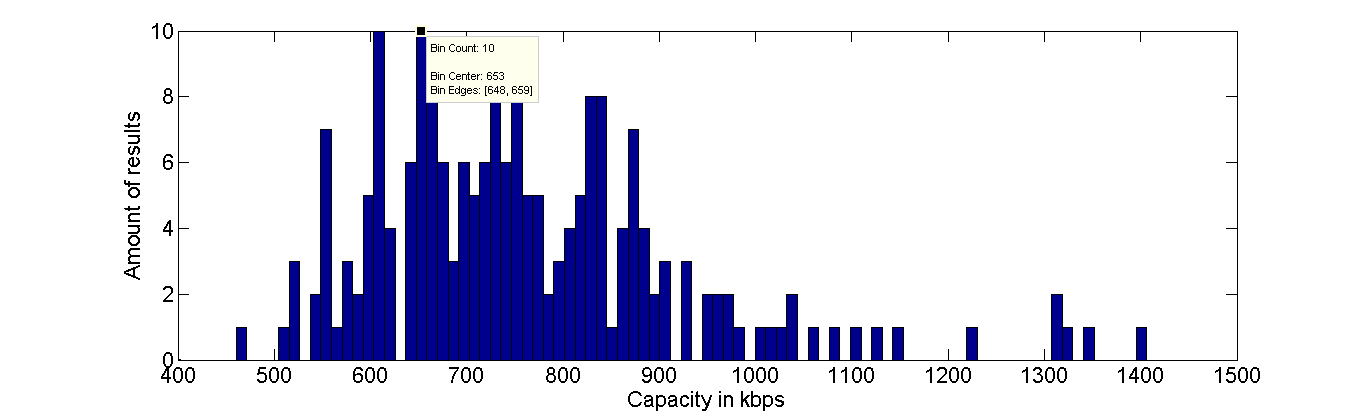
\includegraphics[width=\textwidth]{bilder/histogram_packet_size_200C.png}
\caption{Histogram of Bottleneck Link from a measurement with packet size of 200 bytes}
\label{bild:200}
\end{figure}

\begin{figure}[!ht]
\centering
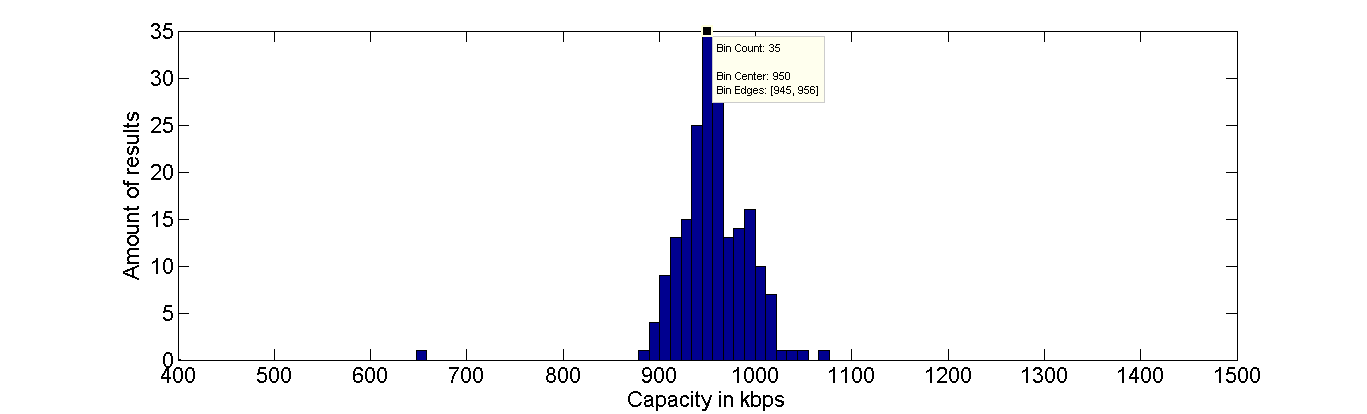
\includegraphics[width=\textwidth]{bilder/histogram_packet_size_1500C.png}
\caption{Histogram of Bottleneck Link from a measurement with packet size of 1500 bytes}
\label{bild:1500}
\end{figure}

\begin{figure}[!ht]
\centering
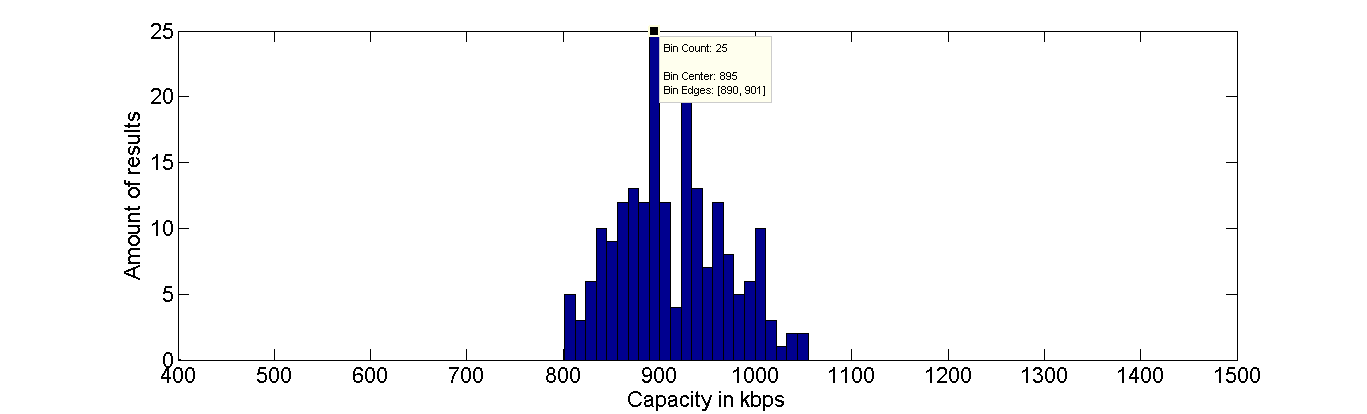
\includegraphics[width=\textwidth]{bilder/histogram_packet_size_800C.png}
\caption{Histogram of Bottleneck Link from a measurement with packet size of 800 bytes}
\label{bild:800}
\end{figure}

The results with the packet size of 200 bytes show large noise. Consequently the exact value for the bottleneck link cannot be seen. As discussed in the lecture, this is due to high probability of cross traffic for small packet sizes. The lowest noise is shown with the large packets. The size of 1500 bytes is the bound to have non-fragmented packets. So it is the maximum possible packet size to get reliable results. There it can be said, that the link rate is approximately 950 kbps. This is a logical value due to a DSL connection which has a 1024 kbps rate. With large packet sizes it is unlikely to have cross traffic. However if there is cross traffic with large packet sizes the influences for the results are a lot higher than with small packets, because the time interval between the packet pair is larger, in which the cross traffic could get into account. As illustrated, with a high amount of measurements, this effect can be disregarded. Additionally with large packets the time difference is also larger, which is easier to measure due to rounding errors.

Normally the value for packet size to get the best accurate result is between these two sizes, like 800 bytes. Consequently, the probability and the influence of cross traffic are both relatively low. However, there does not exist an optimal value for packet size in general. A minimum packet size is needed due to precision of measurements of the computer. Consequently for high data rate, large packet sizes are necessary to measure the time exactly. In this case, the results with 800 bytes display more noise than the large packet size.  On this account the packet size of 1500 bytes seems to be suitable and consequently the bottleneck link rate is 950 kbps.


%
%\let\clearpage\relax
%
\chapter{\label{text:Kap4}Conclusions}
This report showed an implementation of a method to measure the bottleneck link rate. There, a timeout function was considered and the right value of the bottleneck link rate was decided to be 950 kbps. Good measurements were detected with a packet size of 1500 bytes. Another option to increase the performance of this implementation would be to check the right order of the two packets. This order can be changed with UDP connection and the measurement of the time difference is wrong. Additionally, it could be considered to check plausibility of the results. For example, if the link rate was measured earlier to be a 1024 kbps DSL connection, capacities of 20000 kbps should be categorized to be implausible. Consequently a maximum bound could be created based on former measurements and known information about the network. Another option to get more accurate results is to adapt the histogram accuracy.